\documentclass[12pt]{article}
\usepackage{amsmath}
\usepackage{tikz}
\usepackage{pgfplots}
\usepackage{enumitem}

\title{Introduction to Linear Algebra}\\
\author{Tutoring Centre Ferndale\\
\includegraphics[width=4em]{ApS_logo.png}}
\date{}

\begin{document}

\maketitle

\section*{Linear Equations}

A linear equation is an equation that describes a straight line when its solutions are plotted on a graph. There are three common forms of linear equations:

\subsection*{Standard Form}

The standard form of a linear equation is given by:
\[
Ax + By = C
\]
where:
\begin{itemize}
    \item \( A \), \( B \), and \( C \) are constants.
    \item \( x \) and \( y \) are variables.
\end{itemize}

\subsection*{Slope-Intercept Form}

The slope-intercept form of a linear equation is given by:

$y = mx + b$

where:
\begin{itemize}
    \item \( y \) is the dependent variable (the output value).
    \item \( x \) is the independent variable (the input value).
    \item \( m \) represents the slope of the line.
    \item \( b \) is the y-intercept, which is the point where the line crosses the y-axis.
\end{itemize}

\section*{Point-Slope Form}

In the point-slope form, \(y - y_1 = m(x - x_1)\):
\begin{itemize}
    \item \((x_1, y_1)\) is a point on the line.
    \item \(m\) is the slope of the line.
\end{itemize}

\section*{Graphs of Linear Equations}

\begin{figure}[h!]
    \centering
    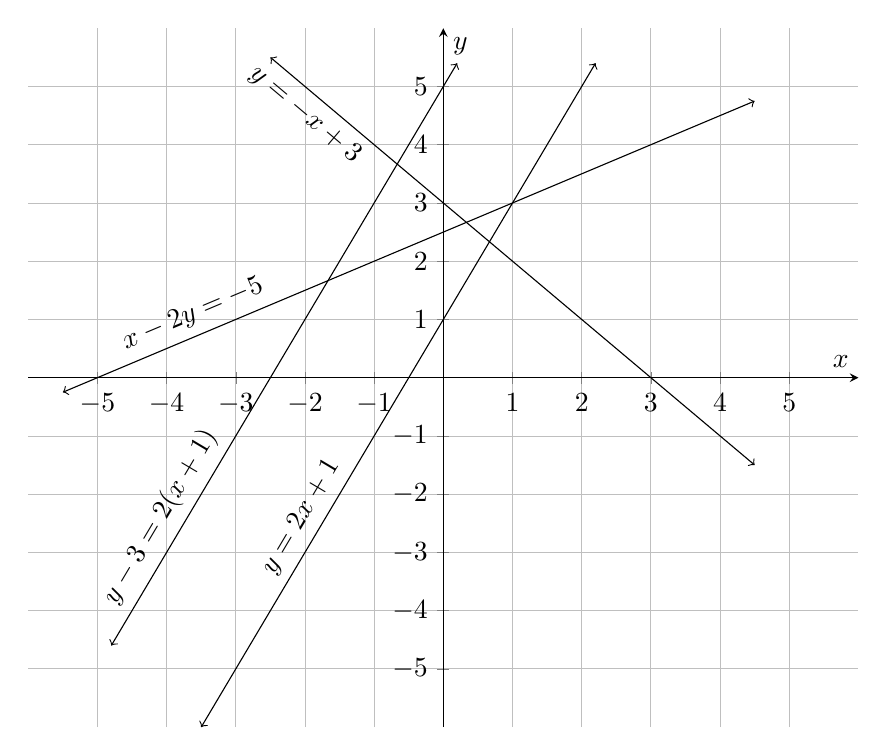
\begin{tikzpicture}
    \begin{axis}[width=\textwidth,
        axis lines = middle,
        xlabel = {$x$},
        ylabel = {$y$},
        xmin=-6, xmax=6,
        ymin=-6, ymax=6,
        xtick={-5,-4,-3,-2,-1,0,1,2,3,4,5},
        ytick={-5,-4,-3,-2,-1,0,1,2,3,4,5},
        grid=both,
        grid style={line width=.3pt, draw=gray!50}]
    \addplot[<->,domain=-3.5:2.2]{2*x + 1} node [pos=0.3,sloped,above]{$y=2x + 1$};
    \addplot[<->,domain=-2.5:4.5]{-1*x + 3} node [pos=0.1,sloped,below]{$y=-x + 3$};
    \addplot[<->,domain=-4.8:0.2]{2*x + 5} node [pos=0.2,sloped,above]{$y - 3 = 2(x + 1)$};
    \addplot[<->,domain=-5.5:4.5]{0.5*x + 2.5} node [pos=0.2,sloped,above]{$x-2y=-5$};
    \end{axis}
\end{tikzpicture}
\end{figure}

Can you identify the forms of the linear equations that are plotted here?

\section*{Effects of Changing Values}

\subsection*{Changing the slope \( m \):}
\begin{itemize}
    \item A positive slope means the line rises from left to right.
    \item A negative slope means the line falls from left to right.
    \item A larger absolute value of the slope means a steeper line.
\end{itemize}

\subsection*{Changing the y-intercept \( b \):}
\begin{itemize}
    \item Increases in \( b \) shift the line up.
    \item Decreases in \( b \) shift the line down.
\end{itemize}

\section*{Practice Problems}

Solve the following real-world problems using linear equations:

\subsection*{Problem 1}

A taxi company charges a base fare of \$3 and an additional \$2 per mile driven. Write the linear equation representing the total fare \( y \) in terms of the number of miles \( x \) driven. Calculate the total fare for a 5-mile trip.\\

\textbf{Solution:}

\[
y = 2x + 3
\]

For \( x = 5 \):

\[
y = 2(5) + 3 = 10 + 3 = 13
\]

\textbf{Total fare:} \$13

\newpage

\subsection*{Problem 2}

A plant grows at a constant rate. After 2 weeks, the plant is 10 cm tall, and after 5 weeks, it is 25 cm tall. Write the linear equation representing the height \( y \) of the plant in terms of the number of weeks \( x \). Determine the height of the plant after 8 weeks.\\

\textbf{Solution:}

First, find the slope \( m \):

\[
m = \frac{\Delta y}{\Delta x} = \frac{25 - 10}{5 - 2} = \frac{15}{3} = 5
\]

Using the point-slope form \( y - y_1 = m(x - x_1) \) and point (2, 10):

\[
y - 10 = 5(x - 2)
\]

Simplify to slope-intercept form:

\[
y - 10 = 5x - 10
\]

\[
y = 5x
\]

For \( x = 8 \):

\[
y = 5(8) = 40
\]

\textbf{Height after 8 weeks:} 40 cm\\

\section*{Conclusion}

Linear algebra provides the tools to describe and analyze linear relationships. Understanding the forms of linear equations, their graphs, and the effects of changing values helps solve real-world problems. Practice with these problems to strengthen your understanding of linear equations and their applications.

\end{document}
